% SAR imaging pipeline figure (TikZ).
% Coordinates in drawio-style px (1 unit = 0.02 cm, y pointing down). Requires tikz.
% Usage: \resizebox{<width>}{!}{% SAR imaging pipeline figure (TikZ).
% Coordinates in drawio-style px (1 unit = 0.02 cm, y pointing down). Requires tikz.
% Usage: \resizebox{<width>}{!}{% SAR imaging pipeline figure (TikZ).
% Coordinates in drawio-style px (1 unit = 0.02 cm, y pointing down). Requires tikz.
% Usage: \resizebox{<width>}{!}{% SAR imaging pipeline figure (TikZ).
% Coordinates in drawio-style px (1 unit = 0.02 cm, y pointing down). Requires tikz.
% Usage: \resizebox{<width>}{!}{\input{../figures/pipeline/sar_imaging_pipeline.tex}}
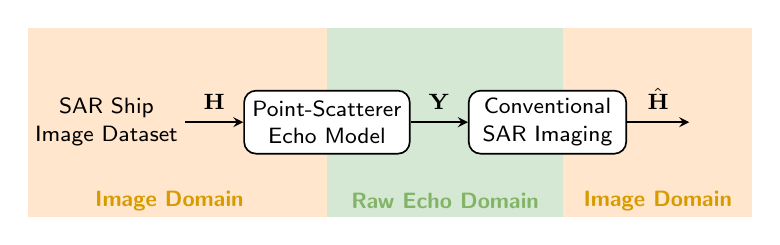
\begin{tikzpicture}[
    x=0.02cm, y=-0.02cm,
    font=\fontsize{8.5}{10}\linespread{1}\selectfont\sffamily,
    line width=0.6pt,
    box/.style={draw, rounded corners=1.5mm, minimum width=2cm, minimum height=0.8cm,
                inner xsep=3pt, inner ysep=2pt, align=center},
    lbl/.style={align=center, inner sep=0pt},
    flow/.style={-stealth},
  ]
  \definecolor{efOrange}{HTML}{FFE6CC}
  \definecolor{efGreen}{HTML}{D5E8D4}
  \definecolor{efOrangeText}{HTML}{D79B00}
  \definecolor{efGreenText}{HTML}{82B366}

  % Domain backgrounds
  \fill[efOrange] (160,80) rectangle (350,200);
  \fill[efGreen]  (350,80) rectangle (500,200);
  \fill[efOrange] (500,80) rectangle (620,200);
  \node[lbl, text=efOrangeText, font=\fontsize{8.5}{10}\linespread{1}\selectfont\sffamily\bfseries] at (250,190) {Image Domain};
  \node[lbl, text=efGreenText,  font=\fontsize{8.5}{10}\linespread{1}\selectfont\sffamily\bfseries] at (425,190) {Raw Echo Domain};
  \node[lbl, text=efOrangeText, font=\fontsize{8.5}{10}\linespread{1}\selectfont\sffamily\bfseries] at (560,190) {Image Domain};

  % Blocks
  \node[lbl]             (data) at (210,140) {SAR Ship\\Image Dataset};
  \node[box, fill=white] (echo) at (350,140) {Point-Scatterer\\Echo Model};
  \node[box, fill=white] (img)  at (490,140) {Conventional\\SAR Imaging};

  % Flow
  \draw[flow] (260,140) -- (echo.west) node[midway, above=1pt] {$\mathbf{H}$};
  \draw[flow] (echo.east) -- (img.west) node[midway, above=1pt] {$\mathbf{Y}$};
  \draw[flow] (img.east) -- (580,140) node[midway, above=1pt] {$\hat{\mathbf{H}}$};
\end{tikzpicture}
}
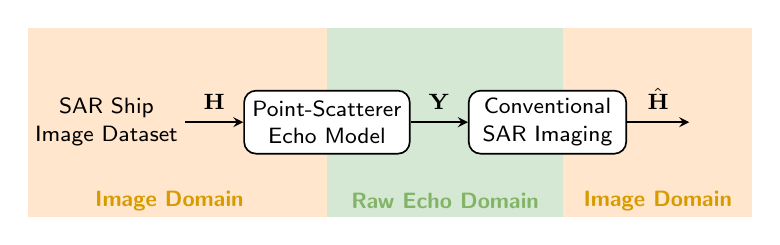
\begin{tikzpicture}[
    x=0.02cm, y=-0.02cm,
    font=\fontsize{8.5}{10}\linespread{1}\selectfont\sffamily,
    line width=0.6pt,
    box/.style={draw, rounded corners=1.5mm, minimum width=2cm, minimum height=0.8cm,
                inner xsep=3pt, inner ysep=2pt, align=center},
    lbl/.style={align=center, inner sep=0pt},
    flow/.style={-stealth},
  ]
  \definecolor{efOrange}{HTML}{FFE6CC}
  \definecolor{efGreen}{HTML}{D5E8D4}
  \definecolor{efOrangeText}{HTML}{D79B00}
  \definecolor{efGreenText}{HTML}{82B366}

  % Domain backgrounds
  \fill[efOrange] (160,80) rectangle (350,200);
  \fill[efGreen]  (350,80) rectangle (500,200);
  \fill[efOrange] (500,80) rectangle (620,200);
  \node[lbl, text=efOrangeText, font=\fontsize{8.5}{10}\linespread{1}\selectfont\sffamily\bfseries] at (250,190) {Image Domain};
  \node[lbl, text=efGreenText,  font=\fontsize{8.5}{10}\linespread{1}\selectfont\sffamily\bfseries] at (425,190) {Raw Echo Domain};
  \node[lbl, text=efOrangeText, font=\fontsize{8.5}{10}\linespread{1}\selectfont\sffamily\bfseries] at (560,190) {Image Domain};

  % Blocks
  \node[lbl]             (data) at (210,140) {SAR Ship\\Image Dataset};
  \node[box, fill=white] (echo) at (350,140) {Point-Scatterer\\Echo Model};
  \node[box, fill=white] (img)  at (490,140) {Conventional\\SAR Imaging};

  % Flow
  \draw[flow] (260,140) -- (echo.west) node[midway, above=1pt] {$\mathbf{H}$};
  \draw[flow] (echo.east) -- (img.west) node[midway, above=1pt] {$\mathbf{Y}$};
  \draw[flow] (img.east) -- (580,140) node[midway, above=1pt] {$\hat{\mathbf{H}}$};
\end{tikzpicture}
}
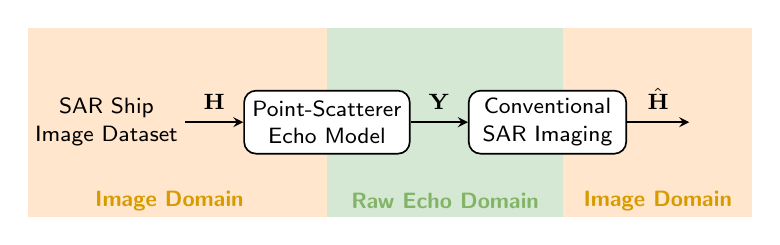
\begin{tikzpicture}[
    x=0.02cm, y=-0.02cm,
    font=\fontsize{8.5}{10}\linespread{1}\selectfont\sffamily,
    line width=0.6pt,
    box/.style={draw, rounded corners=1.5mm, minimum width=2cm, minimum height=0.8cm,
                inner xsep=3pt, inner ysep=2pt, align=center},
    lbl/.style={align=center, inner sep=0pt},
    flow/.style={-stealth},
  ]
  \definecolor{efOrange}{HTML}{FFE6CC}
  \definecolor{efGreen}{HTML}{D5E8D4}
  \definecolor{efOrangeText}{HTML}{D79B00}
  \definecolor{efGreenText}{HTML}{82B366}

  % Domain backgrounds
  \fill[efOrange] (160,80) rectangle (350,200);
  \fill[efGreen]  (350,80) rectangle (500,200);
  \fill[efOrange] (500,80) rectangle (620,200);
  \node[lbl, text=efOrangeText, font=\fontsize{8.5}{10}\linespread{1}\selectfont\sffamily\bfseries] at (250,190) {Image Domain};
  \node[lbl, text=efGreenText,  font=\fontsize{8.5}{10}\linespread{1}\selectfont\sffamily\bfseries] at (425,190) {Raw Echo Domain};
  \node[lbl, text=efOrangeText, font=\fontsize{8.5}{10}\linespread{1}\selectfont\sffamily\bfseries] at (560,190) {Image Domain};

  % Blocks
  \node[lbl]             (data) at (210,140) {SAR Ship\\Image Dataset};
  \node[box, fill=white] (echo) at (350,140) {Point-Scatterer\\Echo Model};
  \node[box, fill=white] (img)  at (490,140) {Conventional\\SAR Imaging};

  % Flow
  \draw[flow] (260,140) -- (echo.west) node[midway, above=1pt] {$\mathbf{H}$};
  \draw[flow] (echo.east) -- (img.west) node[midway, above=1pt] {$\mathbf{Y}$};
  \draw[flow] (img.east) -- (580,140) node[midway, above=1pt] {$\hat{\mathbf{H}}$};
\end{tikzpicture}
}
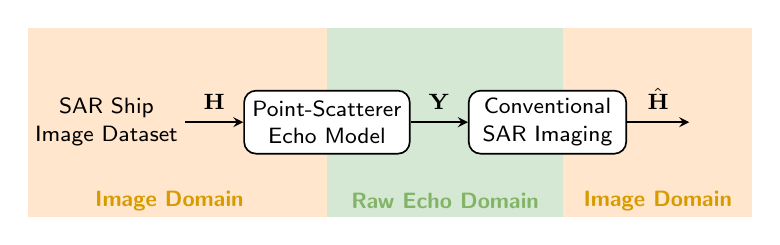
\begin{tikzpicture}[
    x=0.02cm, y=-0.02cm,
    font=\fontsize{8.5}{10}\linespread{1}\selectfont\sffamily,
    line width=0.6pt,
    box/.style={draw, rounded corners=1.5mm, minimum width=2cm, minimum height=0.8cm,
                inner xsep=3pt, inner ysep=2pt, align=center},
    lbl/.style={align=center, inner sep=0pt},
    flow/.style={-stealth},
  ]
  \definecolor{efOrange}{HTML}{FFE6CC}
  \definecolor{efGreen}{HTML}{D5E8D4}
  \definecolor{efOrangeText}{HTML}{D79B00}
  \definecolor{efGreenText}{HTML}{82B366}

  % Domain backgrounds
  \fill[efOrange] (160,80) rectangle (350,200);
  \fill[efGreen]  (350,80) rectangle (500,200);
  \fill[efOrange] (500,80) rectangle (620,200);
  \node[lbl, text=efOrangeText, font=\fontsize{8.5}{10}\linespread{1}\selectfont\sffamily\bfseries] at (250,190) {Image Domain};
  \node[lbl, text=efGreenText,  font=\fontsize{8.5}{10}\linespread{1}\selectfont\sffamily\bfseries] at (425,190) {Raw Echo Domain};
  \node[lbl, text=efOrangeText, font=\fontsize{8.5}{10}\linespread{1}\selectfont\sffamily\bfseries] at (560,190) {Image Domain};

  % Blocks
  \node[lbl]             (data) at (210,140) {SAR Ship\\Image Dataset};
  \node[box, fill=white] (echo) at (350,140) {Point-Scatterer\\Echo Model};
  \node[box, fill=white] (img)  at (490,140) {Conventional\\SAR Imaging};

  % Flow
  \draw[flow] (260,140) -- (echo.west) node[midway, above=1pt] {$\mathbf{H}$};
  \draw[flow] (echo.east) -- (img.west) node[midway, above=1pt] {$\mathbf{Y}$};
  \draw[flow] (img.east) -- (580,140) node[midway, above=1pt] {$\hat{\mathbf{H}}$};
\end{tikzpicture}
